\documentclass[11pt]{article}
\usepackage[margin=1in]{geometry}
\usepackage[T1]{fontenc}
\usepackage[utf8]{inputenc}
\usepackage{lmodern}
\usepackage{microtype}
\usepackage{amsmath,amssymb}
\usepackage{graphicx}
\usepackage{booktabs}
\usepackage{adjustbox}
\usepackage[font=small,labelfont=bf]{caption}
\usepackage{enumitem}
\usepackage[colorlinks=true,linkcolor=black,citecolor=black,urlcolor=blue]{hyperref}
\setlist{nosep,leftmargin=*}
\graphicspath{{figures/}}
% let pages hold more and larger floats, so figures stay near their text
\renewcommand{\topfraction}{0.85}
\renewcommand{\textfraction}{0.1}
\renewcommand{\floatpagefraction}{0.75}
\newcommand{\pct}[1]{$#1\%$}

\title{Interpretable Carbon-Aware Electricity Pricing:\\ From Demand Prediction to Tariff Prescription}
\author{Clement Docteur and Panle Chen\\[2pt]
\small 15.095 Machine Learning Under a Modern Optimization Lens --- Final Report}
\date{December 2026}

\begin{document}
\maketitle

\begin{abstract}
\noindent Can an interpretable, carbon-aware pricing policy reduce household electricity emissions relative to a
historical time-of-use (TOU) tariff at a comparable average price? We answer this on the Low Carbon London 2013 trial
(1,032 households on a dynamic tariff) with a three-step pipeline: a next-day forecast of grid carbon intensity,
a demand-response simulator validated on held-out tariff events, and an optimal prescriptive tree that picks each
day's price schedule from a small menu under an average-price constraint. Emissions are counted with marginal emission
factors estimated from the 2013 grid. On the unseen test period (Nov--Dec 2013) a depth-1 policy tree lowers estimated
emissions by \pct{0.90} of the households' footprint (simulator bootstrap \pct{0.80}--\pct{1.01}), against a
hindsight ceiling of \pct{0.97}; direct optimisation finds the same schedules, so interpretability costs nothing.
The saving comes from evening conservation, not from shifting load to clean hours: a carbon-only rule that ignores
demand response \emph{raises} emissions by \pct{1.68}. A time-average price cap does not protect bills (\pct{+9.2}).
Over four rolling test windows the fixed tree falls short in summer; adding the remaining price budget as a tree input
brings it to \pct{-0.59} on average against a ceiling of \pct{-0.62}.
\end{abstract}

% ===================================================================================================================
\section{Introduction}

The carbon intensity (CI) of electricity varies within the day with the generation mix, but conventional TOU tariffs
follow fixed schedules that need not match low-carbon periods. Evidence from the Low Carbon London (LCL) trial shows that
households respond to dynamic prices, mainly by cutting use during High-price periods~\cite{schofield2015,schofield2016}.
Combining carbon forecasts with a model of this response could therefore yield tariffs that cut emissions, provided the
pricing rule stays simple enough for a utility or regulator to audit.

\paragraph{Research question.} Can an interpretable, carbon-aware pricing policy reduce estimated household
electricity emissions relative to the historical 2013 TOU tariff while keeping a comparable average price?

\paragraph{Approach and contributions.} Following our proposal, we (i) forecast next-day half-hourly CI with
regularised regression and tree ensembles; (ii) simulate household consumption under alternative schedules;
(iii) learn an optimal policy tree~\cite{amram2022,bertsimas2019} that maps decision-time features to one of a few
daily schedules, with the price constraint handled by a Lagrangian penalty and an online feasibility rule. Relative to
the proposal we made three substantive changes, each motivated by the data: emissions are counted at the
\emph{margin} rather than with average intensity (Section~\ref{sec:mef}); the CVAE simulator of Br\'eg\`ere and
Bessa~\cite{bregere2020} is replaced as the main simulator by a response model with a flat-tariff control, which
matches held-out events (Section~\ref{sec:sim}); and a \emph{budget-aware} tree is added after a rolling evaluation
exposed a weakness of the fixed tree (Section~\ref{sec:rolling}).

% ===================================================================================================================
\section{Data and Setup}

\textbf{Households.} We use the 1,032 LCL households on the 2013 dynamic TOU tariff that have more than 95\% of their
2013 half-hourly readings~\cite{lcl}. Households differ widely in when they use power, so we group them into four
consumption clusters (285, 299, 299 and 149 households) taken from our reproduction of~\cite{bregere2020}
(Figure~\ref{fig:data}a): cluster~1 has a sharp evening peak, cluster~2 uses more at night, cluster~3 uses the least.
LCL also metered 1,032 households who stayed on a flat tariff (``Std'', 14.228~p/kWh) and therefore saw no price events.
They share the TOU households' weather, holidays and seasons, which makes them a natural control group for measuring
the effect of prices.

\textbf{Tariff.} On any half-hour the TOU price was Low (3.99~p/kWh), Normal (11.76) or High (67.20). High and Low
prices came in blocks of a few hours, announced the day before; 2013 had 73 days with a High block and 93 with a Low
block, spread over the year (Figure~\ref{fig:data}b). We use the trial authors' schedule, aligned to the meter
half-hours. \textbf{Grid.} NESO half-hourly CI and generation mix, 2009--2013~\cite{neso}. \textbf{Weather.} ERA5
2\,m temperature for central London~\cite{era5}.

\textbf{Timing and splits.} The schedule for day $d$ is announced at 12:00 GMT on day $d-1$, so every forecast and
policy input uses only data available at that moment. We split 2013 by time, not at random, so that the test period
is genuinely in the future of everything the models see (Table~\ref{tab:data}). Models, the schedule menu, tree depth
and the Lagrange multiplier are chosen on training and validation data only, and the test period is used once.
\textbf{Price target.} The historical TOU time-average price over Jan--Oct, $\bar p = 13.608$~p/kWh. Because the 2013
tariff averaged only 12.795~p/kWh during the test period, we also report a price-matched variant.

\begin{table}[t]
\centering\small
\caption{Time-based splits of 2013. Event days: days on which the historical tariff had at least one High (or Low)
block. All 1,032 TOU and 1,032 Std households are present in every split.}
\label{tab:data}
\begin{tabular}{llrrrr}
\toprule
Split & Dates & Days & High-event days & Low-event days & Time-avg.\ price (p/kWh) \\
\midrule
Training & Jan--Aug 2013 & 243 & 53 & 61 & 13.63 \\
Validation & Sep--Oct 2013 & 61 & 13 & 14 & 13.52 \\
Test & Nov--Dec 2013 & 61 & 7 & 18 & 12.80 \\
\bottomrule
\end{tabular}
\end{table}

\begin{figure}[t]
\centering
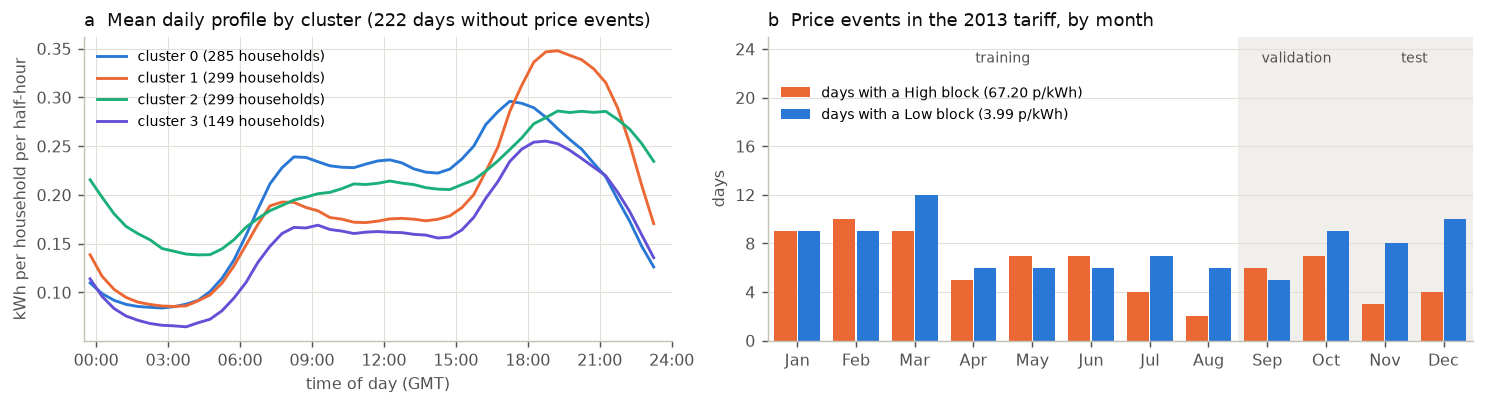
\includegraphics[width=\textwidth]{data_overview.png}
\caption{The data. (a) Mean daily consumption of each household cluster on the 222 days of 2013 without price events.
(b) Days with a High or Low block in the historical 2013 tariff, by month, with the training, validation and test
periods.}
\label{fig:data}
\end{figure}

\textbf{Emission accounting.} A schedule $z$ changes consumption $y_{dh}$ in half-hour $h$ of day $d$; its emissions
change is $\Delta E(z) = \tfrac{1}{1000}\sum_{d,h} \mathrm{MEF}_{dh}\,(\hat y_{dh}(z) - y_{dh})$ kg CO$_2$, reported as
a share of the households' historical footprint at average intensity (298.2~kg per household over the test period).

% ===================================================================================================================
\section{Methods}

Figure~\ref{fig:pipeline} summarises the pipeline. Steps~1 and~1b describe the grid: what the carbon intensity will be
tomorrow, and how much CO$_2$ an extra kWh actually causes. Step~2 describes the households: how their consumption
changes under a given price schedule. Step~3 combines the two to choose each day's schedule.

\begin{figure}[t]
\centering
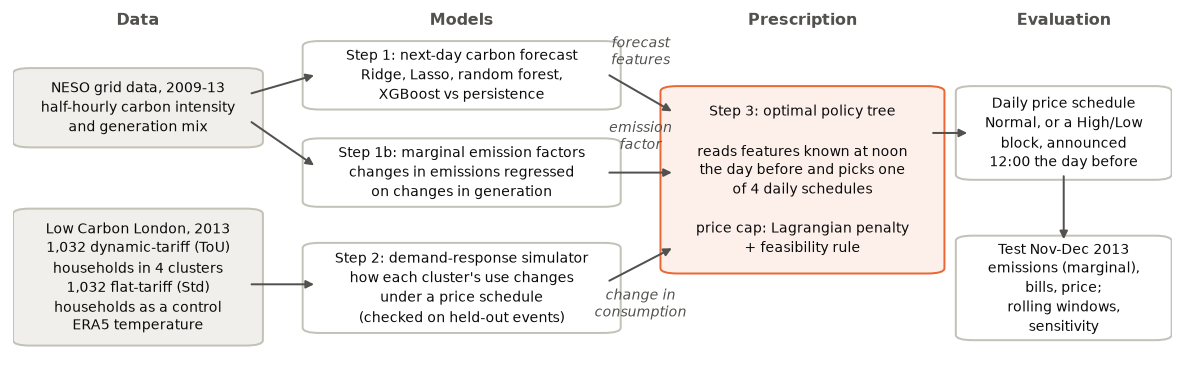
\includegraphics[width=\textwidth]{pipeline.png}
\caption{The three-step pipeline. Each day, the policy tree reads features known at noon the day before and picks a
price schedule; schedules are scored with the simulator's change in consumption times the marginal emission factor.}
\label{fig:pipeline}
\end{figure}

\subsection{Step 1: next-day carbon-intensity forecast}
Each model predicts the deviation of every half-hour's CI from the mean of the last known 24 hours, using calendar
features, lagged CI (latest known day, 2 and 7 days earlier), lagged fuel shares and generation (horizon 12--36\,h).
We compare Ridge, Lasso, random forest and XGBoost~\cite{xgboost} with persistence (tomorrow looks like the latest
known day), training on NESO data from 2009 with monthly expanding refits and hyperparameters tuned on validation.
On validation the tree ensembles cut the mean absolute error of persistence by 24\% (24.0 vs 31.6~g/kWh) and XGBoost
was selected; on the test period the gain shrinks (XGBoost 27.2, random forest 26.0, persistence 28.4~g/kWh;
Figure~\ref{fig:ci}). The forecasts track the daily level but miss the timing of swings within a day: the rank
correlation between forecast and actual half-hours of the same day is only 0.32 for XGBoost. The most likely reason is
that these swings follow wind output and plant availability, which lagged grid data cannot anticipate; adding
temperature does not help. The forecast enters the policy tree as five daily features (mean, evening mean,
evening-minus-night gap, range, and start of the dirtiest 3-hour window).

\begin{figure}[t]
\centering
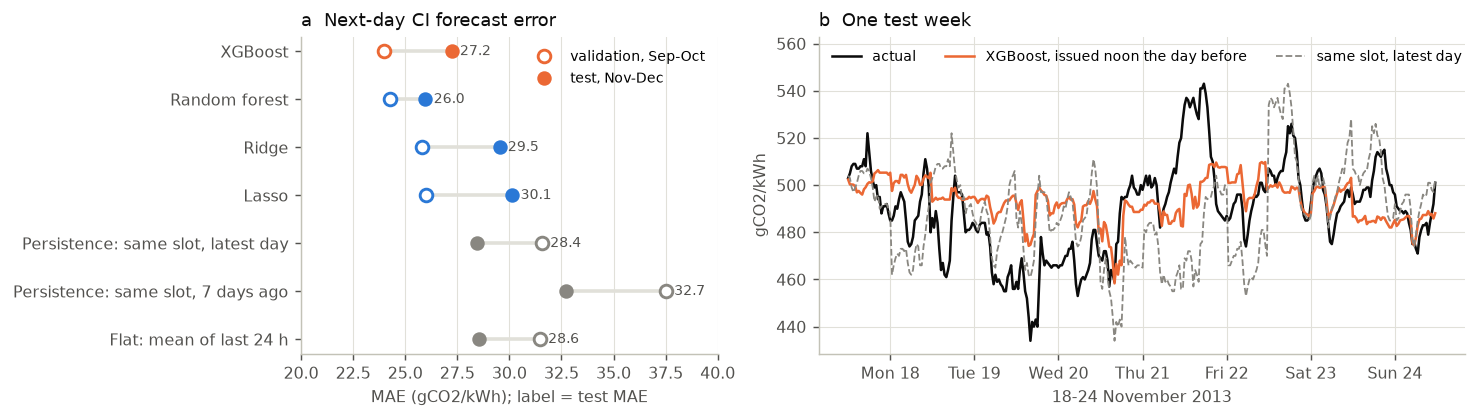
\includegraphics[width=\textwidth]{step1_ci_forecast.png}
\caption{Next-day CI forecasts. (a) Mean absolute error of each model on validation (Sep--Oct) and test (Nov--Dec);
the tree ensembles beat persistence on both, by less on test. (b) One test week: XGBoost, issued at noon the day
before, follows the level of CI but not its sharper swings.}
\label{fig:ci}
\end{figure}

\subsection{Step 1b: marginal emission factors}\label{sec:mef}
A tariff changes demand at the margin, so its emissions depend on the plants that ramp, not on the average mix. For
each hour of day $h$ and season $s$ (Oct--Mar, Apr--Sep) we regress half-hourly changes in system emissions on
changes in generation~\cite{hawkes2010}: $\Delta E_t = \alpha_{hs} + \beta_{hs}\,\Delta G_t + \varepsilon_t$, with
$E_t = \mathrm{CI}_t\,G_t$; the slope $\beta_{hs}$ is the marginal emission factor (MEF). NESO counts pumped-storage
output as zero-carbon, but that energy was pumped overnight, so storage output is charged the overnight MEF divided by
a 75\% round-trip efficiency (930~g/kWh). Factors that \emph{score} schedules are estimated on 2013; factors available
at \emph{decision time} are re-estimated monthly on the previous 12 months.

The 2013 margin looks nothing like the average (Figure~\ref{fig:mef}). Overnight, coal met 58\% of changes in
generation (MEF $\approx 679$~g/kWh); at the evening peak gas met 64\% and pumped storage 17\%, giving 318~g/kWh if
storage is counted as clean but 514~g/kWh once it is charged for overnight coal --- above the average intensity of those
hours (462~g/kWh). The annual marginal factor also fell from 659 (2009) to 462~g/kWh (2013) as gas displaced coal at
the margin, so factors must be estimated close to the period they describe.

\begin{figure}[t]
\centering
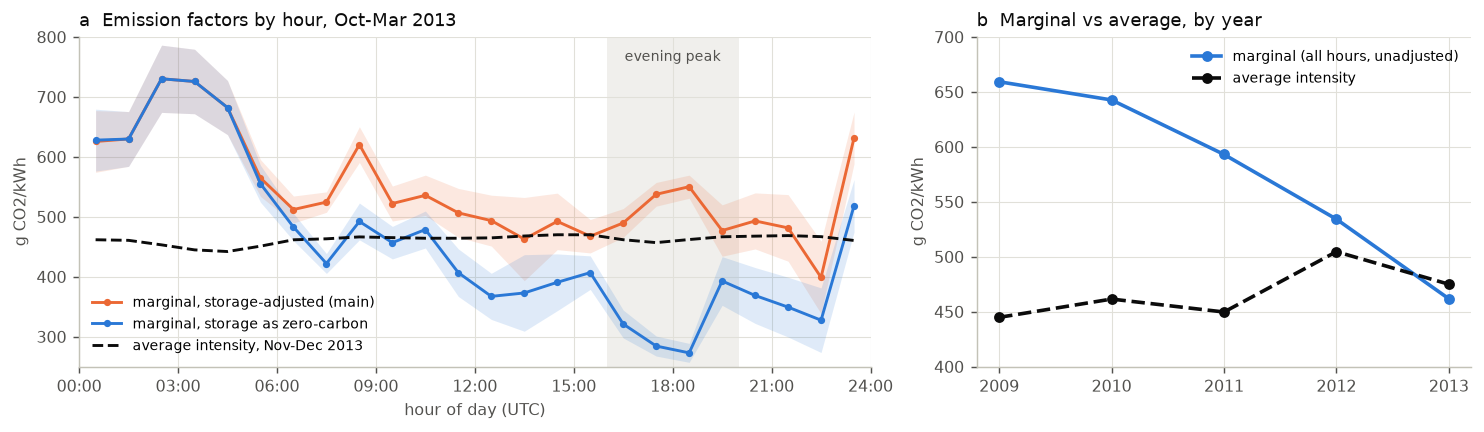
\includegraphics[width=\textwidth]{step1b_marginal_emissions.png}
\caption{Marginal emission factors by hour, Oct--Mar 2013, with and without the pumped-storage adjustment, against the
average intensity of the test period (a); annual marginal factor and average intensity, 2009--2013 (b). Bands:
$\pm 2$ standard errors.}
\label{fig:mef}
\end{figure}

\subsection{Step 2: demand-response simulator}\label{sec:sim}
The proposal planned to adapt the conditional variational autoencoder (CVAE) of~\cite{bregere2020}. Our reproduction
found its mean profiles accurate but its tariff response unreliable: the latent variable collapses, the sign of the
response changes between training runs, and it barely reacts to High prices on held-out days. We keep it as a
sensitivity case and use as main simulator a simpler cluster-level response model. The idea is to compare each TOU
cluster with the flat-tariff households on the same half-hour: anything that affects both groups (weather, holidays,
season) cancels in the ratio, and what remains is the effect of the price. For cluster $c$, the log ratio of ToU to
Std consumption is regressed on slot $\times$ day-type intercepts, temperature terms and tariff regressors $r(z)$:
\[
\log \frac{y^{\text{ToU}}_{cdh}}{y^{\text{Std}}_{cdh}} = \alpha_{c,h,\tau(d)} + \theta_c^\top w_{dh}
 + \gamma_c^\top r(z_d)_h + \varepsilon_{cdh}.
\]
The tariff terms are in-block High and Low effects by time of day (pooled effects plus ridge-shrunk deviations by
time band) and edge effects around blocks, i.e.\ changes in use just before or after a block (households may, for
instance, wait for a Low block to start before running appliances). We compare three specifications on validation
event days: no edge effects; only the three edge effects that our reproduction of~\cite{bregere2020} had found in the
raw data (a 2-hour dip before Low blocks, the half-hour after a Low block, 2 hours before High blocks); and all edge
and day-level terms. The middle one has the lowest validation error and is our main simulator. A schedule's simulated
consumption is the observed consumption times the modelled ratio between that schedule and the historical one,
$\hat y_{cdh}(z) = y_{cdh}\exp\!\big(m_c(z)_{dh} - m_c(z^{\text{hist}})_{dh}\big)$, clipped to $[1/4,4]$, so only the
tariff response is modelled. Inside blocks, cluster~3 cuts use by 29\% under evening High prices and raises it by 49\%
under afternoon Low prices; no other cluster exceeds 6\%. To check the simulator on data it has not seen, we measure
the actual effect of each Nov--Dec event as a difference-in-differences --- the change in TOU consumption during the
block minus the change in Std consumption over the same half-hours --- and compare it with the simulated effect. The
model reproduces these observed effects (e.g.\ High blocks: observed \pct{-7.7}, model \pct{-7.5}, CVAE \pct{-1.1};
Figure~\ref{fig:sim}). Uncertainty is propagated with 200 weekly-block bootstrap refits.

\begin{figure}[t]
\centering
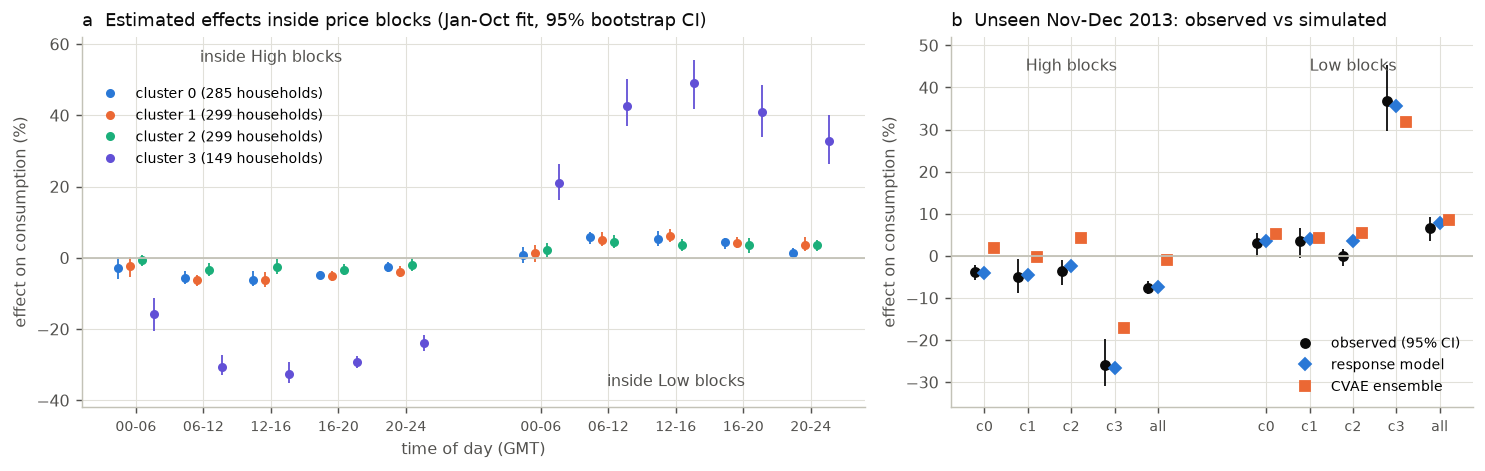
\includegraphics[width=\textwidth]{step2_demand_response.png}
\caption{Estimated in-block tariff effects by cluster (a). On held-out Nov--Dec event days (b) the response model
matches the observed High and Low effects for all households and for cluster 3; the CVAE ensemble barely reacts to
High prices.}
\label{fig:sim}
\end{figure}

\subsection{Step 3: prescriptive policy tree}\label{sec:tree}
\textbf{Actions.} Each day receives one schedule from a menu $\mathcal A$, chosen by greedy forward selection from
98 plausible single-block schedules (High 2--4\,h, Low 3--6\,h, evening High + night Low) on training-day hindsight
costs. The selected menu is: Normal all day (11.76~p/kWh time-average), High 17:00--20:00 (18.69), High 18:00--20:00
(16.38) and Low 02:00--05:00 (10.79).

\textbf{Costs and constraint.} For day $d$ and action $a$, $C_d(a)$ is the simulated emissions change with the 2013
MEFs, and $p(a)$ the schedule's time-average price. The tree $T$ maps decision-time features $x_d$ (CI-forecast
summaries, temperature, weekend/holiday, recent consumption) to a leaf $\ell(x_d)$ that prescribes $a_\ell$:
\[
\min_{T:\ \text{depth}\le D,\ |\ell|\ge 10}\ \sum_{d} \Big[ C_d\big(a_{\ell(x_d)}\big) + \lambda\, p\big(a_{\ell(x_d)}\big)\Big].
\]
The penalty $\lambda$ turns the price constraint into a cost: each p/kWh of time-average price counts as $\lambda$
kg of CO$_2$, so a larger $\lambda$ makes expensive schedules (High blocks) less attractive. We solve this problem
exactly by exhaustive search (all thresholds at the last split, 12 quantile thresholds above), for $D\in\{1,2,3\}$.
The multiplier $\lambda$ is a hyperparameter chosen with $D$ on validation emissions; tuning $\lambda$ to meet the
target on training days made coarse trees spend nothing on new data. Each leaf also stores a ranking of all actions
by summed cost.

\textbf{Feasibility rule.} Over an evaluation period of $N$ days the time-average price must not exceed $\bar p$.
Day $j$ takes the first action in its leaf's ranking such that the target remains attainable if every remaining day
were all-Normal: $\sum_{k\le j} p_k + (N-j)\,p_{\text{Normal}} \le N\bar p$. Once the budget is spent, events are
cancelled. (Using the cheapest schedule as the floor let policies overspend early and then forced Low days, which add
consumption.)

\textbf{Budget-aware tree.} The tree cannot see how much budget is left, so it may waste budget early or leave it
unused. We add one feature, the remaining budget per remaining day above the all-Normal price,
$s_j = (N\bar p - \sum_{k<j} p_k)/(N-j) - p_{\text{Normal}}$. Training data must then cover many budget situations,
not only the one that happened. We therefore copy each fitting day 9 times, once per budget level $s$ from 0 to
9.5~p/kWh. Each copy gets its own price penalty: the $\lambda$ at which picking the best action day by day would, on
average, spend exactly $s$. The tree thus learns which action is best on a given day \emph{and} at a given budget.

\textbf{Baselines.} The historical 2013 TOU schedule; a simple carbon rule (High on the forecast-dirtiest contiguous
window, Low on the cleanest, sized to meet $\bar p$, no demand model); direct optimisation (per day, the action
minimising forecast cost $+\lambda p$, with the same feasibility rule), also with a perfect MEF forecast; a budget-aware
direct optimiser; and a perfect-hindsight oracle (the ceiling for this menu and simulator).

% ===================================================================================================================
\section{Results}

\subsection{Main test period (Nov--Dec 2013)}
The validation-selected tree has depth~1 (Figure~\ref{fig:trees}a, Table~\ref{tab:main}): if recent consumption
(the households' mean use over the week ending two days before) exceeds 0.171~kWh per half-hour, it prescribes High
17:00--20:00, otherwise Normal. Recent consumption marks the darker, colder half of the year, when an evening High
block saves the most; no carbon-forecast feature enters the tree. In the test period the tree asks for
the High block every day, the budget covers 16 of them, and the feasibility rule cancels the rest. The tree lowers
emissions by \pct{0.90} of the footprint (about 2.7~kg CO$_2$ per household over 61 days), against \pct{0.97} for perfect
hindsight. Direct optimisation picks exactly the same schedules, so the interpretable policy loses nothing, and a
perfect MEF forecast changes nothing, because the policy is driven by demand, not by carbon timing.

\begin{table}[t]
\centering\small
\caption{Test period Nov--Dec 2013, 1,032 households, main simulator. Emissions: change in MEF-weighted consumption vs
the historical TOU tariff, \% of the historical footprint; bootstrap: 200 weekly-block refits of the simulator. Prices
in p/kWh; price paid = bill / kWh. ``Adj.'': days on which the feasibility rule overrode the policy.}
\label{tab:main}
\begin{adjustbox}{max width=\textwidth}
\begin{tabular}{lrcrrrrr}
\toprule
Policy & Emissions & 95\% bootstrap & Time-avg. & Paid & Mean bill & Adj. & High/Low \\
 & & & price & price & & & half-hours \\
\midrule
Historical TOU (2013) & 0 & --- & 12.80 & 12.99 & 0 & --- & 90 / 252 \\
Carbon rule (no demand model) & $+1.68\%$ & $[+1.40, +1.94]$ & 13.61 & 11.41 & $-10.6\%$ & --- & 183 / 610 \\
Optimal policy tree & $-0.90\%$ & $[-1.01, -0.80]$ & 13.58 & 14.30 & $+9.2\%$ & 45 & 96 / 0 \\
Direct optimisation & $-0.90\%$ & $[-1.01, -0.80]$ & 13.58 & 14.30 & $+9.2\%$ & 45 & 96 / 0 \\
\quad with perfect MEF forecast & $-0.90\%$ & $[-1.01, -0.80]$ & 13.58 & 14.30 & $+9.2\%$ & 45 & 96 / 0 \\
Budget-aware tree & $-0.93\%$ & $[-1.03, -0.83]$ & 13.57 & 15.00 & $+14.5\%$ & 6 & 124 / 204 \\
Budget-aware direct opt. & $-0.92\%$ & $[-1.00, -0.82]$ & 13.54 & 14.69 & $+12.2\%$ & 5 & 110 / 114 \\
Oracle (hindsight) & $-0.97\%$ & $[-1.06, -0.87]$ & 13.60 & 15.00 & $+14.5\%$ & --- & 118 / 150 \\
\bottomrule
\end{tabular}
\end{adjustbox}
\end{table}

\textbf{The saving is conservation, not shifting.} High prices cut evening use without moving it elsewhere, and the
evening peak is when use is highest; total consumption falls by 0.79\% and the daily peak by 1.9\%. The carbon-only
rule, which places prices by forecast intensity alone, \emph{raises} emissions by \pct{1.68}: following the marginal
factors it puts High prices at night, when few people use power, and Low prices in the afternoon, when the Low-price
response adds far more consumption than the High block removes.

\textbf{Bills rise.} High blocks fall on the evening peak, so at the time-average target the price actually paid rises
from 12.99 to 14.30~p/kWh and the mean bill by 9.2\%. A time-average cap therefore does not protect consumers.

\textbf{Budget-aware tree.} Its depth-2 tree (Figure~\ref{fig:trees}b) first splits on recent consumption, then on
the remaining budget: on low-consumption days it earns budget with the night Low block unless more than 4~p/kWh per
day remains; on high-consumption days it picks the full (17:00--20:00) or shorter (18:00--20:00) evening block
depending on whether more than 1.25~p/kWh remains.

\begin{figure}[t]
\centering
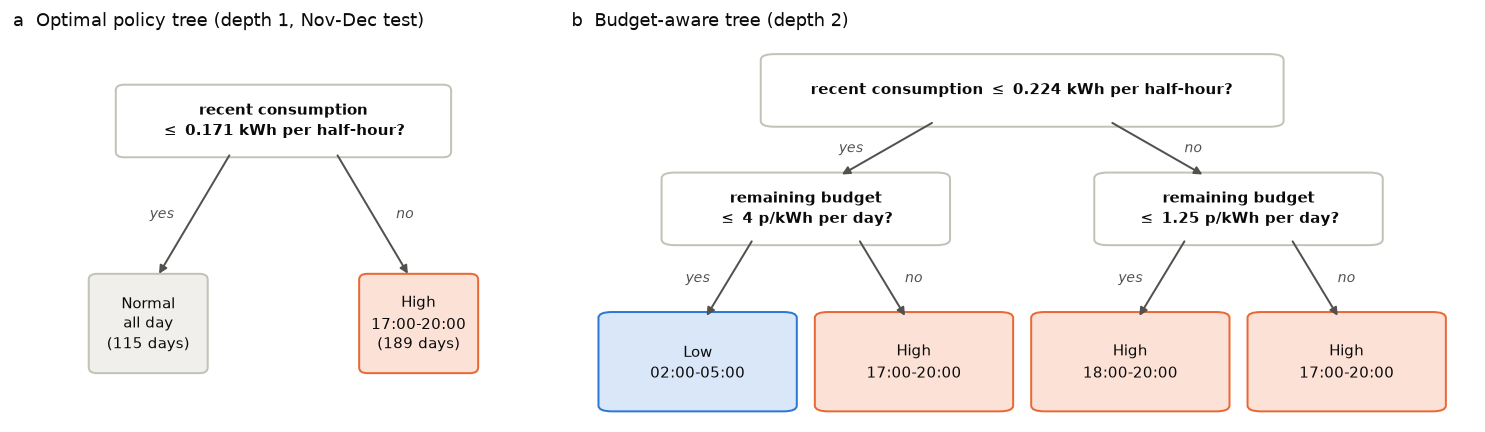
\includegraphics[width=\textwidth]{step3_trees.png}
\caption{The two policies, as they would be handed to a regulator. (a) The validation-selected policy tree; counts are
training and validation days in each leaf. (b) The budget-aware tree, which also reads the remaining price budget per
remaining day (p/kWh above the all-Normal price).}
\label{fig:trees}
\end{figure} In Nov--Dec it ran night Low blocks through November and spent the budget on evening High
blocks in December (Figure~\ref{fig:sched}), saving \pct{0.93} with only 6 rule overrides --- but with a 14.5\% higher
mean bill, since it actually spends the budget.

\begin{figure}[t]
\centering
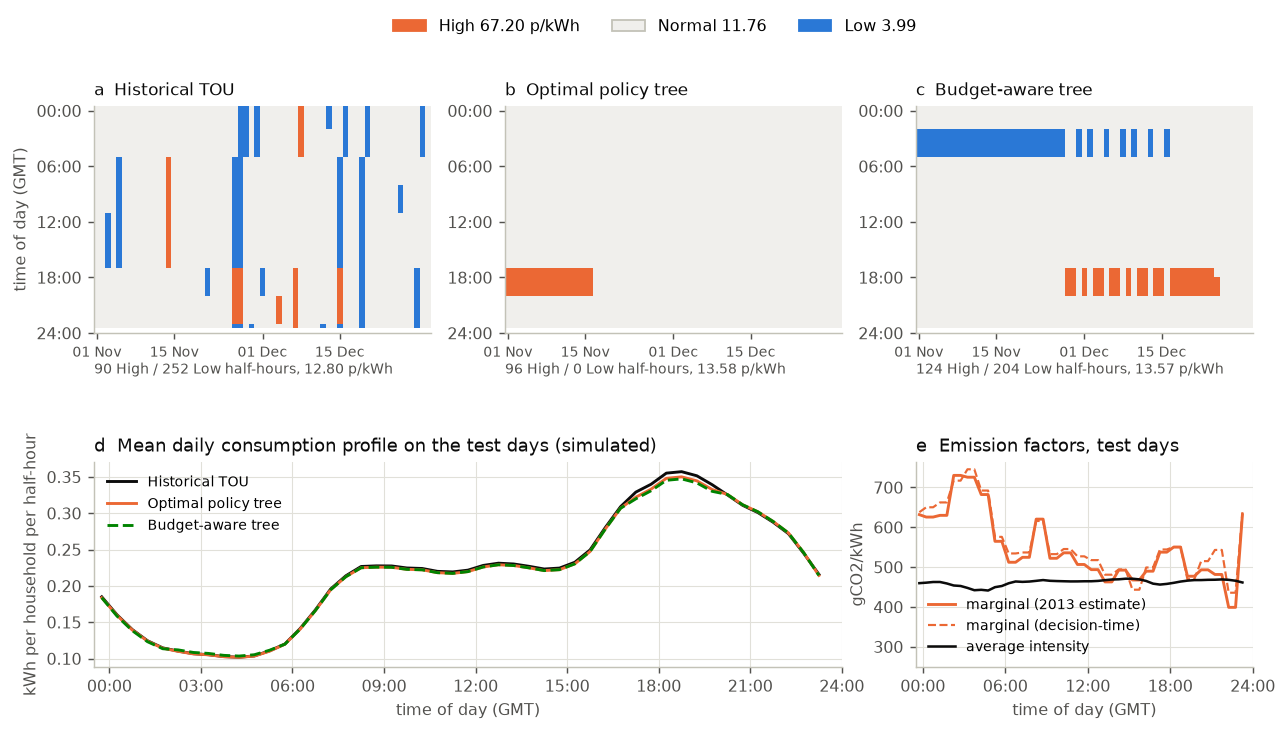
\includegraphics[width=0.92\textwidth]{step3_schedules.png}
\caption{Price schedules over the test period for the historical tariff (a), the policy tree (b) and the budget-aware
tree (c); mean consumption profiles (d); marginal factors vs average intensity over the day (e).}
\label{fig:sched}
\end{figure}

\subsection{Marginal vs average accounting}
Marginal accounting changes the size of the effect, not the policy. Trained on average intensity, the tree prescribes
High 16:00--20:00 and, scored with marginal factors, saves \pct{0.87}; trained on marginal factors it saves \pct{0.90}.
Scored with average intensity the saving is \pct{0.76}: the storage-adjusted evening margin is dirtier than the evening
average. Pumped storage decides the sign of this difference --- counting storage as zero-carbon, as NESO's intensity
does, makes the peak look clean and shrinks the saving to \pct{0.65}. The carbon-only rule is the policy most exposed:
it goes from \pct{+0.18} under average intensity to \pct{+1.68} under marginal factors.

\subsection{Rolling evaluation}\label{sec:rolling}
Because 61 winter days are a narrow test, we repeat the whole protocol on four 2-month windows, each with the
simulator refitted, the menu and hyperparameters chosen only on earlier days, and the target set to the 2013 tariff's own
price in the window (Table~\ref{tab:rolling}). Nov--Dec is the best window for the fixed tree. In May--Jun and Jul--Aug
it never prescribes an event: its consumption threshold is learned on colder months, so every summer day falls on the
Normal side, and in May--Jun, when the 2013 tariff ran many High blocks, it does worse than history. The budget-aware
tree uses that summer budget and averages \pct{-0.59}, close to the hindsight ceiling of \pct{-0.62}. The carbon-only
rule raises emissions in every window.

\begin{table}[t]
\centering\small
\caption{Rolling evaluation, price-matched to the 2013 tariff's time-average price in each window (carbon rule at the
window's own target). Emissions vs historical TOU, marginal factors, \% of footprint. Event days: days with a
non-Normal schedule.}
\label{tab:rolling}
\begin{tabular}{lrrrrrr}
\toprule
Test window & Tree & Tree event days & Budget-aware tree & Its event days & Oracle & Carbon rule \\
\midrule
May--Jun & $+0.10\%$ & 0 & $-0.64\%$ & 42 & $-0.68\%$ & $+2.14\%$ \\
Jul--Aug & $-0.32\%$ & 0 & $-0.42\%$ & 6 & $-0.43\%$ & $+0.92\%$ \\
Sep--Oct & $-0.55\%$ & 23 & $-0.58\%$ & 23 & $-0.62\%$ & $+1.85\%$ \\
Nov--Dec & $-0.71\%$ & 9 & $-0.73\%$ & 55 & $-0.76\%$ & $+1.68\%$ \\
\midrule
Mean & $-0.37\%$ & & $-0.59\%$ & & $-0.62\%$ & $+1.65\%$ \\
\bottomrule
\end{tabular}
\end{table}

\subsection{Sensitivity}
Table~\ref{tab:sens} varies the price constraint and the simulator. About 22\% of the main saving comes from spending
a larger budget than the 2013 tariff did in Nov--Dec: price-matched, the tree saves \pct{0.71} with a bill change of
only \pct{+0.6}. Capping the average price \emph{paid} instead of the time-average limits the bill increase to 4.0\%
while saving \pct{0.78}. Savings scale almost proportionally with the strength of the response. Under the CVAE,
which barely responds to High prices, the main tree's saving vanishes (\pct{-0.01}); re-trained on the CVAE, the tree
reaches \pct{-0.49}. The budget-aware tree trained on the main simulator is fragile in that world (\pct{+8.52}),
most likely because its night Low blocks add consumption that the CVAE's weak High response does not offset;
re-trained on the CVAE it saves \pct{0.56}.

\begin{table}[t]
\centering\small
\caption{Sensitivity, Nov--Dec 2013. Top: price constraints (main simulator; $\lambda$ re-chosen on validation).
Bottom: simulated worlds; ``main'' policies are trained on the main simulator and evaluated in each world,
``re-trained'' ones are trained in that world.}
\label{tab:sens}
\begin{adjustbox}{max width=\textwidth}
\begin{tabular}{lrrrr}
\toprule
Price constraint & Tree & Budget-aware tree & Oracle & Tree bill \\
\midrule
Time-avg.\ $\le 12.795$ (2013 tariff, test period) & $-0.71\%$ & $-0.73\%$ & $-0.76\%$ & $+0.6\%$ \\
Time-avg.\ $\le 13.517$ (full-year 2013, proposal) & $-0.87\%$ & $-0.91\%$ & $-0.94\%$ & $+8.0\%$ \\
Time-avg.\ $\le 13.608$ (Jan--Oct 2013; main) & $-0.90\%$ & $-0.93\%$ & $-0.97\%$ & $+9.2\%$ \\
Time-avg.\ $\le 14.228$ (flat Std tariff) & $-1.06\%$ & $-1.10\%$ & $-1.13\%$ & $+16.4\%$ \\
Price paid $\le 13.784$ (Jan--Oct 2013) & $-0.78\%$ & $-0.81\%$ & $-0.83\%$ & $+4.0\%$ \\
\midrule
Simulated world & Main tree & Main budget-aware & Tree re-trained & Oracle \\
\midrule
Response $\times 0.5$ & $-0.49\%$ & $-0.51\%$ & $-0.49\%$ & $-0.53\%$ \\
Response $\times 1.5$ & $-1.25\%$ & $-1.28\%$ & $-1.25\%$ & $-1.34\%$ \\
Full model (+ post-block, day-level terms) & $-0.83\%$ & $-1.14\%$ & $-1.16\%$ & $-1.19\%$ \\
CVAE ensemble (proposal's simulator) & $-0.01\%$ & $+8.52\%$ & $-0.49\%$ & $-0.76\%$ \\
\bottomrule
\end{tabular}
\end{adjustbox}
\end{table}

\textbf{Solver check.} We planned to use Interpretable AI's Optimal Policy Trees~\cite{amram2022}, which could not run
in our computing environment; our solver approximates the upper splits with 12 quantile thresholds. Refitting all 24
trees of the study (four windows, fixed and budget-aware, depths 1--3) with every threshold at every level (the exact
optimum for depth $\le 2$) or 24 thresholds (depth 3), our search attains 98--100\% of the optimum's training gain, and
the finer trees never improve a test result. Four of the eight selected trees, including the main one, have depth 1,
where the search is exact.

% ===================================================================================================================
\section{Discussion and Limitations}

The pipeline answers the research question with a qualified yes: a one-split tree, readable by any regulator, cuts
estimated household emissions by about 1\% at the same time-average price as the 2013 tariff, which is close to what
any policy over this menu can achieve given how the trial households responded. Three lessons stand out.
\emph{First}, demand response, not carbon timing, drives the result: the households' main lever is cutting evening
use, and CI-forecast features enter only one of the eight selected trees (the depth-3 Sep--Oct tree). \emph{Second}, how emissions are counted matters more for
carbon-only rules than for demand-aware policies; at the 2013 margin, pricing by intensity alone backfires.
\emph{Third}, the constraint must match the policy goal: a time-average cap lets bills rise by 9\%, and a policy that
does not see its remaining budget wastes it in summer.

\textbf{Limitations.} All counterfactual emissions are model-based: the response model matches held-out in-block and
edge effects, but new schedules combine effects estimated from 2013 events, and the CVAE world shows the result is
sensitive to the simulator. Marginal factors are short-run statistical estimates that ignore transmission losses and
long-run effects on investment, and the storage adjustment assumes 75\% efficiency and overnight pumping. Each test
window is only two months, the early rolling windows have short histories, and the bootstrap covers simulator
uncertainty in the main window only. Households are represented by four clusters, so bill changes assume each household
responds like its cluster. Temperature enters as realised values, and wind --- a main driver of CI swings --- is not in
the data.

% ===================================================================================================================
\section{Conclusion}

An interpretable prescriptive tree, trained on a validated demand-response simulator and evaluated with marginal
emission factors, reduces the estimated emissions of 1,032 London households by \pct{0.90} in the test period,
essentially matching direct optimisation and coming within 0.07 points of perfect hindsight. Making the tree aware of
its remaining price budget extends this performance across the year (\pct{-0.59} vs a ceiling of \pct{-0.62}). The
gains are modest and come with higher bills.

\paragraph{Future work.} Several extensions follow directly from these results. (i)~\emph{Protecting bills}: richer
menus with bill-neutral schedules or rebates, and a constraint on the price actually paid rather than the time-average
price. (ii)~\emph{Targeting}: the four clusters respond very differently (cluster~3 by far the most), so schedules
chosen per cluster, or per household, could save more at the same price. (iii)~\emph{Carbon timing}: CI forecasts
miss most within-day swings; adding wind and plant-availability forecasts could make carbon features useful to the
tree. (iv)~\emph{A cleaner grid}: on the 2013 grid the margin was coal and gas at most hours; with more renewables
today, the gap between clean and dirty hours is likely wider, and carbon timing may matter more than it did here.
(v)~\emph{Solver}: fitting Interpretable AI's Optimal Policy Trees on the exported training sets, on a machine where
the package runs, would confirm our solver check.

\paragraph{Reproducibility.} All results are produced by the scripts in \texttt{carbon\_tariff\_pipeline/}
(about 35 minutes end to end on a laptop), which also generate a detailed HTML report with every table.

% ===================================================================================================================
\section*{Contributions}
% TODO: replace the bracketed text with who did what (the example report from last year has one short paragraph).
\textbf{[To be completed: who did the data preparation and the CVAE reproduction, the carbon forecast and marginal
emission factors, the demand-response simulator, the policy trees and their evaluation, and the writing of the
report.]}

% ===================================================================================================================
\begin{thebibliography}{99}\small
\bibitem{amram2022} M.~Amram, J.~Dunn and Y.~D.~Zhuo. Optimal policy trees. \emph{Machine Learning}, 111:2741--2768, 2022.
\bibitem{bertsimas2019} D.~Bertsimas and J.~Dunn. \emph{Machine Learning Under a Modern Optimization Lens}. Dynamic Ideas, 2019.
\bibitem{bregere2020} M.~Br\'eg\`ere and R.~J.~Bessa. Simulating tariff impact in electrical energy consumption profiles
with conditional variational autoencoders. \emph{IEEE Access}, 8:131949--131966, 2020.
\bibitem{xgboost} T.~Chen and C.~Guestrin. XGBoost: a scalable tree boosting system. In \emph{Proc.\ KDD}, 785--794, 2016.
\bibitem{hawkes2010} A.~D.~Hawkes. Estimating marginal CO$_2$ emissions rates for national electricity systems.
\emph{Energy Policy}, 38(10):5977--5987, 2010.
\bibitem{era5} H.~Hersbach et al. The ERA5 global reanalysis. \emph{Quarterly Journal of the Royal Meteorological
Society}, 146:1999--2049, 2020.
\bibitem{neso} National Energy System Operator. Historic generation mix and carbon intensity.
\url{https://www.neso.energy/data-portal/historic-generation-mix}.
\bibitem{schofield2015} J.~Schofield, R.~Carmichael, S.~Tindemans, M.~Woolf, M.~Bilton and G.~Strbac. Experimental
validation of residential consumer responsiveness to dynamic time-of-use pricing. \emph{CIRED}, 2015.
\bibitem{schofield2016} J.~R.~Schofield, S.~H.~Tindemans and G.~Strbac. A baseline-free method to identify responsive
customers on dynamic time-of-use tariffs. arXiv:1605.08078, 2016.
\bibitem{lcl} UK Power Networks. SmartMeter energy consumption data in London households. London Datastore.
\url{https://data.london.gov.uk/dataset/smartmeter-energy-consumption-data-in-london-households}.
\end{thebibliography}

\end{document}
